\section{Écarts à la planification}
\label{sec:ecarts}

Durant l'implémentation de Glasir, plusieurs évènements ont impacté la planification initialement prévue du projet. Pour rendre compte de cela, les diagrammes de Gantt d'avant et d'après l'implémentation sont respectivement présentés à la {\sc figure}~\ref{fig:planifInit} et à la {\sc figure}~\ref{fig:planif}. Les sous-sections ci-après détaillent les changements majeurs du point de vue de la planification du projet. 

\subsection{Gestion du temps}
\label{ssec:temps}

L'un des premiers constats que l'on peut énoncer maintenant que l'implémentation est terminée, est que nous avions de manière générale légèrement surévalué la durée des tâches. Il est possible de le remarquer en comparant la {\sc figure}~\ref{fig:planifInit} (planification initiale) et la {\sc figure}~\ref{fig:planif} (adaptation de la planification suite au développement). Cette surévaluation a cependant permis de gagner du temps, qui a ensuite été utilisé pour améliorer certaines fonctionnalités du logiciel ou bien pour en créer de nouvelles. Ce gain de temps a également permis de surmonter les difficultés rencontrées sans trop prendre de retard.

Ainsi, nous avons pu gérer la sauvegarde de plus d'une modification de l'arbre dans ADTool, ce qui a permis l'annulation de plusieurs actions, au lieu d'une seule comme annoncé initialement.

Le temps supplémentaire a également permis d'autres améliorations mineures, comme le nommage des fenêtre, mais a surtout permis de développer un \og view mode \fg{} pour ADTool. Son intérêt est expliqué plus tard, dans la {\sc section}~\ref{sec:decisions}.

Enfin, ce gain de temps a aidé à gérer les difficultés imprévues rencontrées lors de l'élaboration des algorithmes des modules principaux de Glasir, et ce sans faire prendre de retard au projet. Nous avons même été en mesure de fournir une version plus intelligente du Filtre que celle qui était prévue, puisqu'elle est capable de trouver les n\oe{}uds incorrects en-dessous des n\oe{}uds conjonctifs.

\subsection{Décisions d'implémentation}
\label{sec:decisions}

Malgré le gain de temps évoqué dans la {\sc sous-section}~\ref{ssec:temps}, nous avons tout de même été confrontés à des difficultés que nous n'avons pas pu gérer. Deux éléments du logiciel initialement prévus ont en effet dûs être abandonnés : l'affichage multi-paramètres dans ADTool, et l'intégration complète d'ADTool au sein de Glasir.

L'affichage multi-paramètres, que nous estimions être une fonctionnalité relativement simple à implémenter, s'est avérée très complexe après l'étude approfondie du code source d'ADTool. En effet, l'implémentation de cette fonctionnalité aurait nécessité de réorganiser l'intégralité du code, ce qui n'était pas possible au vu du temps imparti dans le cadre de ce projet. 

L'intégration complète d'ADTool au sein de Glasir a quant à elle été abandonnée, malgré de nombreuses tentatives. Nous n'avons simplement pas réussi à trouver des méthodes permettant l'exécution d'un thread Java au sein d'un processus C\#. Pour remédier à cette impasse, une version \og view mode \fg d'ADTool a été mise au point, dans laquelle toutes les fonctionnalités de création et de modification d'ADTrees sont désactivées. Cela permet d'utiliser ADTool en tant que processus extérieur à Glasir, sans craindre des incohérences dûes à des modifications d'arbres sous ADTool ignorées de Glasir.  

    \begin{figure}[H]
        \centering
        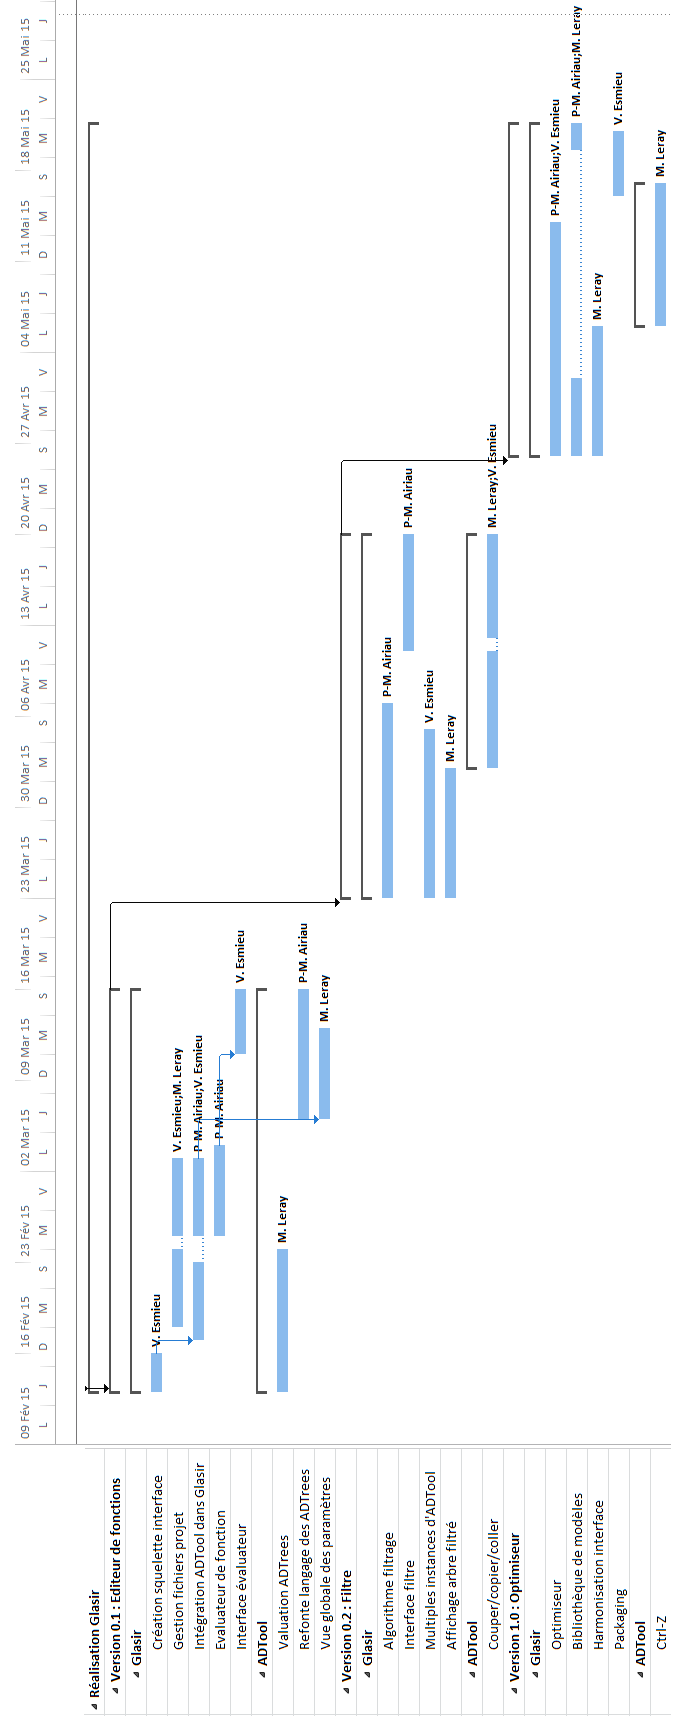
\includegraphics[height=1.6\textwidth]{figure/planifInit.png}
        \caption{Diagramme de Gantt au début du projet Glasir.}
        \label{fig:planifInit}
    \end{figure}

    \begin{figure}[H]
        \centering
        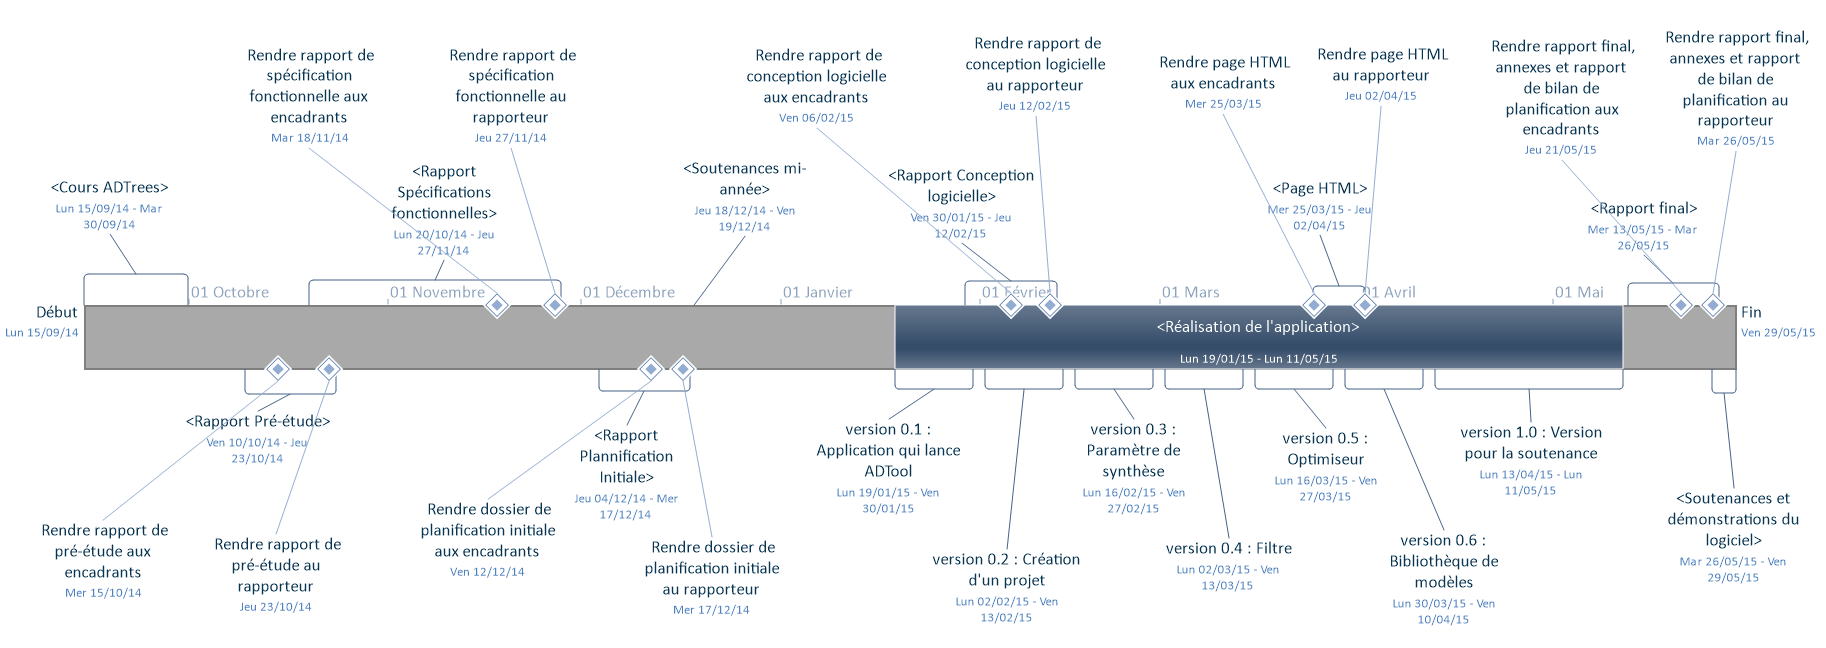
\includegraphics[height=1.6\textwidth]{figure/planification.png}
        \caption{Diagramme de Gantt à la fin du projet Glasir.}
        \label{fig:planif}
    \end{figure}





